% Options for packages loaded elsewhere
\PassOptionsToPackage{unicode}{hyperref}
\PassOptionsToPackage{hyphens}{url}
\PassOptionsToPackage{dvipsnames,svgnames,x11names}{xcolor}
%
\documentclass[
]{article}
\usepackage{amsmath,amssymb}
\usepackage{iftex}
\ifPDFTeX
  \usepackage[T1]{fontenc}
  \usepackage[utf8]{inputenc}
  \usepackage{textcomp} % provide euro and other symbols
\else % if luatex or xetex
  \usepackage{unicode-math} % this also loads fontspec
  \defaultfontfeatures{Scale=MatchLowercase}
  \defaultfontfeatures[\rmfamily]{Ligatures=TeX,Scale=1}
\fi
\usepackage{lmodern}
\ifPDFTeX\else
  % xetex/luatex font selection
\fi
% Use upquote if available, for straight quotes in verbatim environments
\IfFileExists{upquote.sty}{\usepackage{upquote}}{}
\IfFileExists{microtype.sty}{% use microtype if available
  \usepackage[]{microtype}
  \UseMicrotypeSet[protrusion]{basicmath} % disable protrusion for tt fonts
}{}
\makeatletter
\@ifundefined{KOMAClassName}{% if non-KOMA class
  \IfFileExists{parskip.sty}{%
    \usepackage{parskip}
  }{% else
    \setlength{\parindent}{0pt}
    \setlength{\parskip}{6pt plus 2pt minus 1pt}}
}{% if KOMA class
  \KOMAoptions{parskip=half}}
\makeatother
\usepackage{xcolor}
\usepackage[margin=1in]{geometry}
\usepackage{color}
\usepackage{fancyvrb}
\newcommand{\VerbBar}{|}
\newcommand{\VERB}{\Verb[commandchars=\\\{\}]}
\DefineVerbatimEnvironment{Highlighting}{Verbatim}{commandchars=\\\{\}}
% Add ',fontsize=\small' for more characters per line
\usepackage{framed}
\definecolor{shadecolor}{RGB}{248,248,248}
\newenvironment{Shaded}{\begin{snugshade}}{\end{snugshade}}
\newcommand{\AlertTok}[1]{\textcolor[rgb]{0.94,0.16,0.16}{#1}}
\newcommand{\AnnotationTok}[1]{\textcolor[rgb]{0.56,0.35,0.01}{\textbf{\textit{#1}}}}
\newcommand{\AttributeTok}[1]{\textcolor[rgb]{0.13,0.29,0.53}{#1}}
\newcommand{\BaseNTok}[1]{\textcolor[rgb]{0.00,0.00,0.81}{#1}}
\newcommand{\BuiltInTok}[1]{#1}
\newcommand{\CharTok}[1]{\textcolor[rgb]{0.31,0.60,0.02}{#1}}
\newcommand{\CommentTok}[1]{\textcolor[rgb]{0.56,0.35,0.01}{\textit{#1}}}
\newcommand{\CommentVarTok}[1]{\textcolor[rgb]{0.56,0.35,0.01}{\textbf{\textit{#1}}}}
\newcommand{\ConstantTok}[1]{\textcolor[rgb]{0.56,0.35,0.01}{#1}}
\newcommand{\ControlFlowTok}[1]{\textcolor[rgb]{0.13,0.29,0.53}{\textbf{#1}}}
\newcommand{\DataTypeTok}[1]{\textcolor[rgb]{0.13,0.29,0.53}{#1}}
\newcommand{\DecValTok}[1]{\textcolor[rgb]{0.00,0.00,0.81}{#1}}
\newcommand{\DocumentationTok}[1]{\textcolor[rgb]{0.56,0.35,0.01}{\textbf{\textit{#1}}}}
\newcommand{\ErrorTok}[1]{\textcolor[rgb]{0.64,0.00,0.00}{\textbf{#1}}}
\newcommand{\ExtensionTok}[1]{#1}
\newcommand{\FloatTok}[1]{\textcolor[rgb]{0.00,0.00,0.81}{#1}}
\newcommand{\FunctionTok}[1]{\textcolor[rgb]{0.13,0.29,0.53}{\textbf{#1}}}
\newcommand{\ImportTok}[1]{#1}
\newcommand{\InformationTok}[1]{\textcolor[rgb]{0.56,0.35,0.01}{\textbf{\textit{#1}}}}
\newcommand{\KeywordTok}[1]{\textcolor[rgb]{0.13,0.29,0.53}{\textbf{#1}}}
\newcommand{\NormalTok}[1]{#1}
\newcommand{\OperatorTok}[1]{\textcolor[rgb]{0.81,0.36,0.00}{\textbf{#1}}}
\newcommand{\OtherTok}[1]{\textcolor[rgb]{0.56,0.35,0.01}{#1}}
\newcommand{\PreprocessorTok}[1]{\textcolor[rgb]{0.56,0.35,0.01}{\textit{#1}}}
\newcommand{\RegionMarkerTok}[1]{#1}
\newcommand{\SpecialCharTok}[1]{\textcolor[rgb]{0.81,0.36,0.00}{\textbf{#1}}}
\newcommand{\SpecialStringTok}[1]{\textcolor[rgb]{0.31,0.60,0.02}{#1}}
\newcommand{\StringTok}[1]{\textcolor[rgb]{0.31,0.60,0.02}{#1}}
\newcommand{\VariableTok}[1]{\textcolor[rgb]{0.00,0.00,0.00}{#1}}
\newcommand{\VerbatimStringTok}[1]{\textcolor[rgb]{0.31,0.60,0.02}{#1}}
\newcommand{\WarningTok}[1]{\textcolor[rgb]{0.56,0.35,0.01}{\textbf{\textit{#1}}}}
\usepackage{graphicx}
\makeatletter
\def\maxwidth{\ifdim\Gin@nat@width>\linewidth\linewidth\else\Gin@nat@width\fi}
\def\maxheight{\ifdim\Gin@nat@height>\textheight\textheight\else\Gin@nat@height\fi}
\makeatother
% Scale images if necessary, so that they will not overflow the page
% margins by default, and it is still possible to overwrite the defaults
% using explicit options in \includegraphics[width, height, ...]{}
\setkeys{Gin}{width=\maxwidth,height=\maxheight,keepaspectratio}
% Set default figure placement to htbp
\makeatletter
\def\fps@figure{htbp}
\makeatother
\setlength{\emergencystretch}{3em} % prevent overfull lines
\providecommand{\tightlist}{%
  \setlength{\itemsep}{0pt}\setlength{\parskip}{0pt}}
\setcounter{secnumdepth}{5}
\usepackage[french]{babel}
\ifLuaTeX
  \usepackage{selnolig}  % disable illegal ligatures
\fi
\usepackage{bookmark}
\IfFileExists{xurl.sty}{\usepackage{xurl}}{} % add URL line breaks if available
\urlstyle{same}
\hypersetup{
  pdfauthor={Khalil Ounis, Manal Derghal, Taqwa Ben Romdhane},
  colorlinks=true,
  linkcolor={Maroon},
  filecolor={Maroon},
  citecolor={Blue},
  urlcolor={blue},
  pdfcreator={LaTeX via pandoc}}

\title{Analyse des algorithmes de Maximum Subarray 1D\\
\strut ~M2 Data Science Algorithmique}
\author{Khalil Ounis, Manal Derghal, Taqwa Ben Romdhane}
\date{Lundi 7 avril 2025}

\begin{document}
\maketitle

{
\hypersetup{linkcolor=}
\setcounter{tocdepth}{2}
\tableofcontents
}
\noindent\hrulefill

\section{Description du problème et
objectif}\label{description-du-probluxe8me-et-objectif}

Le problème du Maximum Subarray 1D consiste à trouver la sous-séquence
contiguë d'un tableau numérique dont la somme des éléments est maximale.
Ce problème classique en algorithmique a des applications en analyse de
données financières, bioinformatique et traitement du signal.

\href{https://en.wikipedia.org/wiki/Maximum_subarray_problem}{La page
Wikipedia du Maximum Subarray} présente plusieurs approches
algorithmiques pour résoudre ce problème. Nous nous concentrons sur deux
méthodes :

\begin{enumerate}
\def\labelenumi{\arabic{enumi}.}
\tightlist
\item
  Algorithme naïf : complexité O(n²)
\item
  Algorithme de Kadane : complexité optimale O(n)
\end{enumerate}

Nos objectifs sont :\\
a. d'implémenter ces algorithmes en R et C++ et évaluer le gain de
temps.\\
b. de confirmer les complexités théoriques par des simulations
intensives.

\begin{center}\rule{0.5\linewidth}{0.5pt}\end{center}

\section{Un premier exemple}\label{un-premier-exemple}

Le package se télécharge ainsi :

\begin{Shaded}
\begin{Highlighting}[]
\NormalTok{devtools}\SpecialCharTok{::}\FunctionTok{install\_github}\NormalTok{(}\StringTok{"AMATERASU11/MaximumSubarray"}\NormalTok{)}
\end{Highlighting}
\end{Shaded}

et ses fonctions sont rendues disponibles sur Rstudio ainsi :

\begin{Shaded}
\begin{Highlighting}[]
\FunctionTok{library}\NormalTok{(MaximumSubarray)}
\end{Highlighting}
\end{Shaded}

On simule un petit exemple d'un vecteur \texttt{v} de taille
\texttt{100}

\begin{Shaded}
\begin{Highlighting}[]
\FunctionTok{set.seed}\NormalTok{(}\DecValTok{123}\NormalTok{)}
\NormalTok{v }\OtherTok{\textless{}{-}} \FunctionTok{sample}\NormalTok{(}\SpecialCharTok{{-}}\DecValTok{100}\SpecialCharTok{:}\DecValTok{100}\NormalTok{, }\DecValTok{100}\NormalTok{, }\AttributeTok{replace =} \ConstantTok{TRUE}\NormalTok{)}
\end{Highlighting}
\end{Shaded}

On teste les 4 algorithmes implémentés avec des noms explicites :

\begin{itemize}
\tightlist
\item
  \texttt{max\_subarray\_sum\_naive}
\item
  \texttt{max\_subarray\_sum\_opt}
\item
  \texttt{max\_subarray\_sum\_naive\_Rcpp}
\item
  \texttt{max\_subarray\_sum\_opt\_Rcpp}
\end{itemize}

Cela donne :

\begin{Shaded}
\begin{Highlighting}[]
\NormalTok{v}
\end{Highlighting}
\end{Shaded}

\begin{verbatim}
##   [1]  58  78 -87  94  69 -51  17 -58 -87  17  52 -11 -10  96 -10  84  -9  36
##  [19]  -2 -29 -75 -94  69  36  63 -23 -20 -58   2  16 -25  42 -69   8 -94  36
##  [37]  68 -27 -78  54  87 -48  34 -48  54  65 -67 -32 -29 -25 -38  40  -4 -10
##  [55]  52 -63 -80 -60  74 -11 -41 -85  15  -7 -95  99 -15 -15 -62  58  17 -51
##  [73] -67 -97 -88 -32  26  52 -49 -79 -12  59 -76 -66  67  11 -71  39  58  20
##  [91]   9  57 -37  41  98 -34  50  21 -22 -16
\end{verbatim}

\begin{Shaded}
\begin{Highlighting}[]
\FunctionTok{max\_subarray\_sum\_naive}\NormalTok{(v)}
\end{Highlighting}
\end{Shaded}

\begin{verbatim}
## $sum
## [1] 329
## 
## $subarray
##  [1]  67  11 -71  39  58  20   9  57 -37  41  98 -34  50  21
\end{verbatim}

\begin{Shaded}
\begin{Highlighting}[]
\FunctionTok{max\_subarray\_sum\_naive\_Rcpp}\NormalTok{(v)}
\end{Highlighting}
\end{Shaded}

\begin{verbatim}
## $sum
## [1] 329
## 
## $subarray
##  [1]  67  11 -71  39  58  20   9  57 -37  41  98 -34  50  21
\end{verbatim}

\begin{Shaded}
\begin{Highlighting}[]
\FunctionTok{max\_subarray\_sum\_opt}\NormalTok{(v)}
\end{Highlighting}
\end{Shaded}

\begin{verbatim}
## $sum
## [1] 329
## 
## $subarray
##  [1]  67  11 -71  39  58  20   9  57 -37  41  98 -34  50  21
\end{verbatim}

\begin{Shaded}
\begin{Highlighting}[]
\FunctionTok{max\_subarray\_sum\_opt\_Rcpp}\NormalTok{(v)}
\end{Highlighting}
\end{Shaded}

\begin{verbatim}
## $sum
## [1] 329
## 
## $subarray
##  [1]  67  11 -71  39  58  20   9  57 -37  41  98 -34  50  21
\end{verbatim}

\begin{center}\rule{0.5\linewidth}{0.5pt}\end{center}

\section{Comparaison R avec C++}\label{comparaison-r-avec-c}

On va faire des comparaisons pour les deux types d'algorithme en R et
C++ pour quantifier leur différence de performance.

La fonction \texttt{one.simu.time} retourne le temps recherché, et
\texttt{one.simu} sera utilisé par \texttt{microbenchmark}, on retourne
le temps en ms

\begin{Shaded}
\begin{Highlighting}[]
\FunctionTok{library}\NormalTok{(microbenchmark)}
\FunctionTok{set.seed}\NormalTok{(}\DecValTok{123}\NormalTok{)}

\NormalTok{one.simu.time }\OtherTok{\textless{}{-}} \ControlFlowTok{function}\NormalTok{(n, func, }\AttributeTok{data\_type =} \StringTok{"random"}\NormalTok{) \{}
  \ControlFlowTok{if}\NormalTok{ (data\_type }\SpecialCharTok{==} \StringTok{"random"}\NormalTok{) \{}
\NormalTok{    v }\OtherTok{\textless{}{-}} \FunctionTok{sample}\NormalTok{(}\SpecialCharTok{{-}}\DecValTok{100}\SpecialCharTok{:}\DecValTok{100}\NormalTok{, n, }\AttributeTok{replace =} \ConstantTok{TRUE}\NormalTok{)}
\NormalTok{  \} }\ControlFlowTok{else} \ControlFlowTok{if}\NormalTok{ (data\_type }\SpecialCharTok{==} \StringTok{"all\_negative"}\NormalTok{) \{}
\NormalTok{    v }\OtherTok{\textless{}{-}} \FunctionTok{sample}\NormalTok{(}\SpecialCharTok{{-}}\DecValTok{100}\SpecialCharTok{:{-}}\DecValTok{1}\NormalTok{, n, }\AttributeTok{replace =} \ConstantTok{TRUE}\NormalTok{)}
\NormalTok{  \} }\ControlFlowTok{else} \ControlFlowTok{if}\NormalTok{ (data\_type }\SpecialCharTok{==} \StringTok{"all\_positive"}\NormalTok{) \{}
\NormalTok{    v }\OtherTok{\textless{}{-}} \FunctionTok{sample}\NormalTok{(}\DecValTok{0}\SpecialCharTok{:}\DecValTok{100}\NormalTok{, n, }\AttributeTok{replace =} \ConstantTok{TRUE}\NormalTok{)}
\NormalTok{  \} }\ControlFlowTok{else}\NormalTok{ \{}
    \FunctionTok{stop}\NormalTok{(}\StringTok{"data\_type inconnu"}\NormalTok{)}
\NormalTok{  \}}

  \ControlFlowTok{if}\NormalTok{ (func }\SpecialCharTok{==} \StringTok{"naive"}\NormalTok{) \{}
\NormalTok{    t }\OtherTok{\textless{}{-}} \FunctionTok{microbenchmark}\NormalTok{(}\FunctionTok{max\_subarray\_sum\_naive}\NormalTok{(v), }\AttributeTok{times =} \DecValTok{1}\NormalTok{)}\SpecialCharTok{$}\NormalTok{time }\SpecialCharTok{/} \FloatTok{1e6}
\NormalTok{  \} }\ControlFlowTok{else} \ControlFlowTok{if}\NormalTok{ (func }\SpecialCharTok{==} \StringTok{"naive\_Rcpp"}\NormalTok{) \{}
\NormalTok{    t }\OtherTok{\textless{}{-}} \FunctionTok{microbenchmark}\NormalTok{(}\FunctionTok{max\_subarray\_sum\_naive\_Rcpp}\NormalTok{(v), }\AttributeTok{times =} \DecValTok{1}\NormalTok{)}\SpecialCharTok{$}\NormalTok{time }\SpecialCharTok{/} \FloatTok{1e6}
\NormalTok{  \} }\ControlFlowTok{else} \ControlFlowTok{if}\NormalTok{ (func }\SpecialCharTok{==} \StringTok{"opt"}\NormalTok{) \{}
\NormalTok{    t }\OtherTok{\textless{}{-}} \FunctionTok{microbenchmark}\NormalTok{(}\FunctionTok{max\_subarray\_sum\_opt}\NormalTok{(v), }\AttributeTok{times =} \DecValTok{1}\NormalTok{)}\SpecialCharTok{$}\NormalTok{time }\SpecialCharTok{/} \FloatTok{1e6}
\NormalTok{  \} }\ControlFlowTok{else} \ControlFlowTok{if}\NormalTok{ (func }\SpecialCharTok{==} \StringTok{"opt\_Rcpp"}\NormalTok{) \{}
\NormalTok{    t }\OtherTok{\textless{}{-}} \FunctionTok{microbenchmark}\NormalTok{(}\FunctionTok{max\_subarray\_sum\_opt\_Rcpp}\NormalTok{(v), }\AttributeTok{times =} \DecValTok{1}\NormalTok{)}\SpecialCharTok{$}\NormalTok{time }\SpecialCharTok{/} \FloatTok{1e6}
\NormalTok{  \} }\ControlFlowTok{else}\NormalTok{ \{}
    \FunctionTok{stop}\NormalTok{(}\StringTok{"fonction inconnue"}\NormalTok{)}
\NormalTok{  \}}

  \FunctionTok{return}\NormalTok{(}\FunctionTok{round}\NormalTok{(t, }\DecValTok{2}\NormalTok{))}
\NormalTok{\}}
\end{Highlighting}
\end{Shaded}

\subsection{Un essai}\label{un-essai}

Sur un exemple, on obtient :

\begin{Shaded}
\begin{Highlighting}[]
\FunctionTok{set.seed}\NormalTok{(}\DecValTok{123}\NormalTok{)}
\NormalTok{n }\OtherTok{\textless{}{-}} \DecValTok{10000}
\FunctionTok{one.simu.time}\NormalTok{(n, }\AttributeTok{func =} \StringTok{"naive"}\NormalTok{)}
\end{Highlighting}
\end{Shaded}

\begin{verbatim}
## [1] 2487.89
\end{verbatim}

\begin{Shaded}
\begin{Highlighting}[]
\FunctionTok{one.simu.time}\NormalTok{(n, }\AttributeTok{func =} \StringTok{"naive\_Rcpp"}\NormalTok{)}
\end{Highlighting}
\end{Shaded}

\begin{verbatim}
## [1] 29.42
\end{verbatim}

\begin{Shaded}
\begin{Highlighting}[]
\FunctionTok{one.simu.time}\NormalTok{(n, }\AttributeTok{func =} \StringTok{"opt"}\NormalTok{)}
\end{Highlighting}
\end{Shaded}

\begin{verbatim}
## [1] 1.11
\end{verbatim}

\begin{Shaded}
\begin{Highlighting}[]
\FunctionTok{one.simu.time}\NormalTok{(n, }\AttributeTok{func =} \StringTok{"opt\_Rcpp"}\NormalTok{)}
\end{Highlighting}
\end{Shaded}

\begin{verbatim}
## [1] 0.13
\end{verbatim}

\subsection{Simulations avec
répétitions}\label{simulations-avec-ruxe9puxe9titions}

On reproduit ces comparaisons de manière plus robuste:

\begin{Shaded}
\begin{Highlighting}[]
\FunctionTok{set.seed}\NormalTok{(}\DecValTok{123}\NormalTok{)}
\NormalTok{nbSimus }\OtherTok{\textless{}{-}} \DecValTok{10}

\NormalTok{time1 }\OtherTok{\textless{}{-}} \FunctionTok{rep}\NormalTok{(}\DecValTok{0}\NormalTok{, nbSimus); time2 }\OtherTok{\textless{}{-}} \FunctionTok{rep}\NormalTok{(}\DecValTok{0}\NormalTok{, nbSimus);}
\NormalTok{time3 }\OtherTok{\textless{}{-}} \FunctionTok{rep}\NormalTok{(}\DecValTok{0}\NormalTok{, nbSimus); time4 }\OtherTok{\textless{}{-}} \FunctionTok{rep}\NormalTok{(}\DecValTok{0}\NormalTok{, nbSimus)}

\ControlFlowTok{for}\NormalTok{(i }\ControlFlowTok{in} \DecValTok{1}\SpecialCharTok{:}\NormalTok{nbSimus)\{time1[i] }\OtherTok{\textless{}{-}} \FunctionTok{one.simu.time}\NormalTok{(n, }\AttributeTok{func =} \StringTok{"naive"}\NormalTok{)\}}
\ControlFlowTok{for}\NormalTok{(i }\ControlFlowTok{in} \DecValTok{1}\SpecialCharTok{:}\NormalTok{nbSimus)\{time2[i] }\OtherTok{\textless{}{-}} \FunctionTok{one.simu.time}\NormalTok{(n, }\AttributeTok{func =} \StringTok{"naive\_Rcpp"}\NormalTok{)\}}
\ControlFlowTok{for}\NormalTok{(i }\ControlFlowTok{in} \DecValTok{1}\SpecialCharTok{:}\NormalTok{nbSimus)\{time3[i] }\OtherTok{\textless{}{-}} \FunctionTok{one.simu.time}\NormalTok{(n, }\AttributeTok{func =} \StringTok{"opt"}\NormalTok{)\}}
\ControlFlowTok{for}\NormalTok{(i }\ControlFlowTok{in} \DecValTok{1}\SpecialCharTok{:}\NormalTok{nbSimus)\{time4[i] }\OtherTok{\textless{}{-}} \FunctionTok{one.simu.time}\NormalTok{(n, }\AttributeTok{func =} \StringTok{"opt\_Rcpp"}\NormalTok{)\}}
\end{Highlighting}
\end{Shaded}

Gain C++ versus R

\begin{Shaded}
\begin{Highlighting}[]
\NormalTok{naive\_speedup\_cpp }\OtherTok{\textless{}{-}} \FunctionTok{mean}\NormalTok{(time1) }\SpecialCharTok{/} \FunctionTok{mean}\NormalTok{(time2)}
\NormalTok{kadane\_speedup\_cpp }\OtherTok{\textless{}{-}} \FunctionTok{mean}\NormalTok{(time3) }\SpecialCharTok{/} \FunctionTok{mean}\NormalTok{(time4)}
\NormalTok{naive\_speedup\_cpp}
\end{Highlighting}
\end{Shaded}

\begin{verbatim}
## [1] 79.13895
\end{verbatim}

\begin{Shaded}
\begin{Highlighting}[]
\NormalTok{kadane\_speedup\_cpp}
\end{Highlighting}
\end{Shaded}

\begin{verbatim}
## [1] 4.864253
\end{verbatim}

Gain naive versus optimisé

\begin{Shaded}
\begin{Highlighting}[]
\NormalTok{kadane\_vs\_naive\_R }\OtherTok{\textless{}{-}} \FunctionTok{mean}\NormalTok{(time1) }\SpecialCharTok{/} \FunctionTok{mean}\NormalTok{(time3)}
\NormalTok{kadane\_vs\_naive\_Rcpp }\OtherTok{\textless{}{-}} \FunctionTok{mean}\NormalTok{(time2) }\SpecialCharTok{/} \FunctionTok{mean}\NormalTok{(time4)}
\NormalTok{kadane\_vs\_naive\_R}
\end{Highlighting}
\end{Shaded}

\begin{verbatim}
## [1] 2163.18
\end{verbatim}

\begin{Shaded}
\begin{Highlighting}[]
\NormalTok{kadane\_vs\_naive\_Rcpp}
\end{Highlighting}
\end{Shaded}

\begin{verbatim}
## [1] 132.9593
\end{verbatim}

On recommence avec \texttt{n\ =\ 20000} seulement pour le gain avec C++
pour Kadane

\begin{Shaded}
\begin{Highlighting}[]
\FunctionTok{set.seed}\NormalTok{(}\DecValTok{123}\NormalTok{)}
\NormalTok{n }\OtherTok{\textless{}{-}} \DecValTok{20000}
\NormalTok{nbSimus }\OtherTok{\textless{}{-}} \DecValTok{10}
\NormalTok{time3 }\OtherTok{\textless{}{-}} \FunctionTok{rep}\NormalTok{(}\DecValTok{0}\NormalTok{, nbSimus); time4 }\OtherTok{\textless{}{-}} \FunctionTok{rep}\NormalTok{(}\DecValTok{0}\NormalTok{, nbSimus)}
\ControlFlowTok{for}\NormalTok{(i }\ControlFlowTok{in} \DecValTok{1}\SpecialCharTok{:}\NormalTok{nbSimus)\{time3[i] }\OtherTok{\textless{}{-}} \FunctionTok{one.simu.time}\NormalTok{(n, }\AttributeTok{func =} \StringTok{"opt"}\NormalTok{)\}}
\ControlFlowTok{for}\NormalTok{(i }\ControlFlowTok{in} \DecValTok{1}\SpecialCharTok{:}\NormalTok{nbSimus)\{time4[i] }\OtherTok{\textless{}{-}} \FunctionTok{one.simu.time}\NormalTok{(n, }\AttributeTok{func =} \StringTok{"opt\_Rcpp"}\NormalTok{)\}}
\NormalTok{median\_kadane\_R\_vs\_Rcpp }\OtherTok{\textless{}{-}} \FunctionTok{median}\NormalTok{(time3) }\SpecialCharTok{/} \FunctionTok{median}\NormalTok{(time4)}
\NormalTok{median\_kadane\_R\_vs\_Rcpp}
\end{Highlighting}
\end{Shaded}

\begin{verbatim}
## [1] 7.215686
\end{verbatim}

\textbf{Conclusion:}

\subsubsection{Performances C++ vs R :}\label{performances-c-vs-r}

\begin{itemize}
\tightlist
\item
  Naïf : C++ 79× plus rapide\\
\item
  Kadane : C++ 5× plus rapide → 7× pour n=20k
\end{itemize}

\subsubsection{Efficacité algorithmique
:}\label{efficacituxe9-algorithmique}

\begin{itemize}
\item
  Kadane 2163× mieux que naïf en R\\
\item
  Kadane 133× mieux que naïf en C++
\item
  Confirme O(n²) naïf vs O(n) Kadane
\end{itemize}

\subsubsection{Recommandations :}\label{recommandations}

\begin{itemize}
\tightlist
\item
  n \textgreater{} 1k : Toujours préférer Kadane\\
\item
  n \textgreater{} 10k : Obligatoire d'utiliser Rcpp\\
\item
  Très grands n : Seul Kadane+Rcpp reste viable
\end{itemize}

\subsection{\texorpdfstring{Simulations avec
\texttt{microbenchmark}}{Simulations avec microbenchmark}}\label{simulations-avec-microbenchmark}

Vous avez besoin des packages \texttt{microbenchmark} et
\texttt{ggplot2} pour exécuter les simulations et afficher les résultats
(sous forme de diagrammes en violon). Nous comparons
\texttt{naive\_Rcpp} avec \texttt{opt\_Rcpp} pour des tailles de données
\texttt{n\ =\ 1000} et \texttt{n\ =\ 10000}.

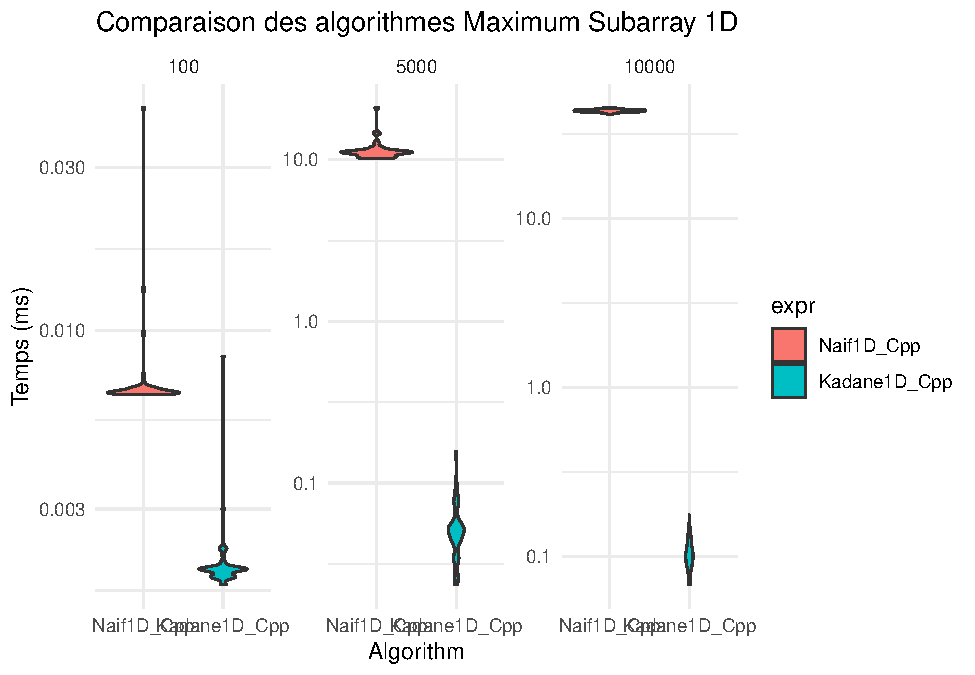
\includegraphics{MaxSubarray1D_files/figure-latex/benchmark-1.pdf}

\begin{verbatim}
## # A tibble: 6 x 8
##       n expr       min_time q1_time median_time mean_time q3_time max_time
##   <dbl> <fct>         <dbl>   <dbl>       <dbl>     <dbl>   <dbl>    <dbl>
## 1   100 Naif_Cpp     0.0041  0.0041      0.0041   0.00459  0.0043   0.0221
## 2   100 Kadane_Cpp   0.0011  0.0012      0.0012   0.00136  0.0013   0.0063
## 3  5000 Naif_Cpp     6.37    6.64        6.88     7.17     7.39    11.7   
## 4  5000 Kadane_Cpp   0.0168  0.0281      0.0310   0.0337   0.0363   0.087 
## 5 10000 Naif_Cpp    25.7    26.4        27.2     27.3     27.8     30.5   
## 6 10000 Kadane_Cpp   0.0441  0.0568      0.0604   0.0642   0.0673   0.118
\end{verbatim}

\begin{center}\rule{0.5\linewidth}{0.5pt}\end{center}

\section{Evaluation de la
complexité}\label{evaluation-de-la-complexituxe9}

Les vecteurs de longueurs \texttt{vector\_n\_naive} et
\texttt{vector\_n\_kadane} (\texttt{n} dans les dataframes) sont choisis
sur l'echelle logarithmique afin d'avoir un pas constant sur l'échelle
logarithmique en abscisse pour la régression.

On réalise 10 répétitions pour chaque valeur de \texttt{n} et pour
chaque algorithme. Les barres d'erreur sont placées en ``mean +/- sd''.

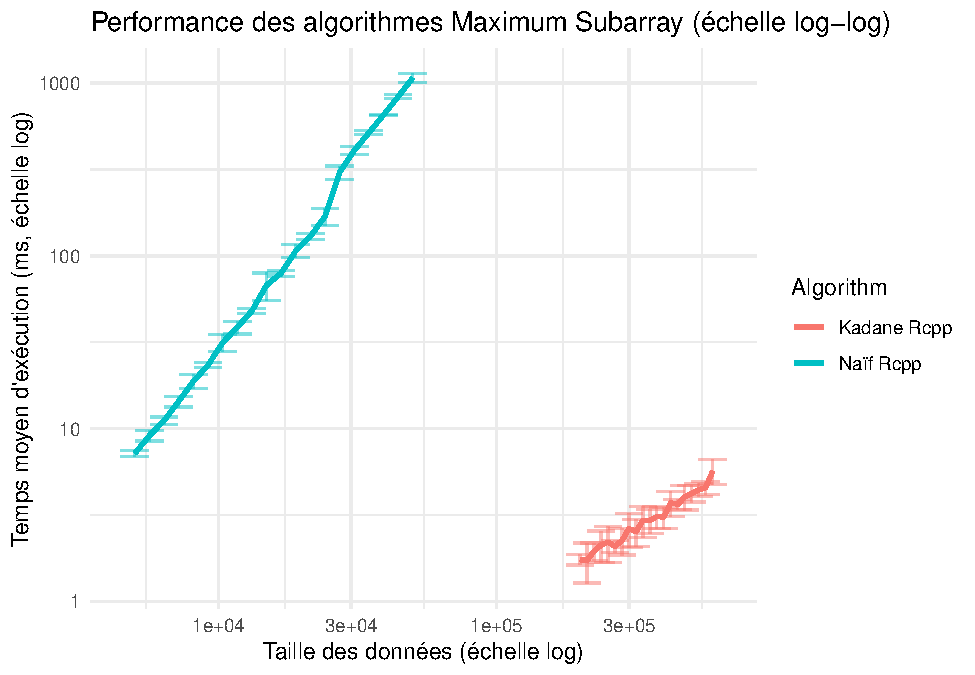
\includegraphics{MaxSubarray1D_files/figure-latex/simu complexite-1.pdf}

\begin{Shaded}
\begin{Highlighting}[]
\CommentTok{\# Affichage des résultats}
\NormalTok{res\_Naive}
\end{Highlighting}
\end{Shaded}

\begin{verbatim}
##        n mean_time    sd_time
## 1   5000     7.089  0.7716713
## 2   5644     8.969  1.0040081
## 3   6371    11.722  1.1311626
## 4   7192    14.360  0.7093189
## 5   8119    18.839  1.1019019
## 6   9165    23.243  1.4850518
## 7  10346    30.953  1.3783569
## 8  11679    37.709  1.5282557
## 9  13183    48.524  1.4181381
## 10 14882    61.565  1.4698772
## 11 16799    81.555 11.3921506
## 12 18963   101.494  3.8724359
## 13 21407   125.332  3.4540244
## 14 24165   161.602  2.9803311
## 15 27278   202.783  2.7031589
## 16 30792   261.185  4.0527748
## 17 34760   332.876  3.7155595
## 18 39238   421.695  5.4820439
## 19 44293   537.211  5.3039827
## 20 50000   686.189  7.9705673
\end{verbatim}

\begin{Shaded}
\begin{Highlighting}[]
\NormalTok{res\_Kadane}
\end{Highlighting}
\end{Shaded}

\begin{verbatim}
##         n mean_time   sd_time
## 1  400000     2.573 0.4202658
## 2  411957     2.526 0.3252076
## 3  424271     2.423 0.2216629
## 4  436953     2.502 0.3260811
## 5  450014     2.573 0.2672514
## 6  463465     2.788 0.2238948
## 7  477319     2.666 0.2424046
## 8  491587     2.676 0.1539264
## 9  506281     2.866 0.2386629
## 10 521415     2.974 0.3452600
## 11 537001     3.090 0.5790605
## 12 553052     3.283 0.5251677
## 13 569584     3.468 0.3315888
## 14 586610     3.363 0.2810318
## 15 604144     3.498 0.3401895
## 16 622203     3.528 0.4707394
## 17 640802     3.794 0.5501555
## 18 659956     3.543 0.1643878
## 19 679683     3.800 0.2701851
## 20 700000     3.828 0.2839718
\end{verbatim}

On vérifie la valeur du coefficient directeur pour les deux méthodes:

\begin{verbatim}
## 
## Call:
## lm(formula = log(res_Naive$mean_time) ~ log(res_Naive$n))
## 
## Residuals:
##       Min        1Q    Median        3Q       Max 
## -0.019263 -0.010687 -0.002297  0.005399  0.035703 
## 
## Coefficients:
##                    Estimate Std. Error t value Pr(>|t|)    
## (Intercept)      -14.922447   0.047727  -312.7   <2e-16 ***
## log(res_Naive$n)   1.982513   0.004924   402.7   <2e-16 ***
## ---
## Signif. codes:  0 '***' 0.001 '**' 0.01 '*' 0.05 '.' 0.1 ' ' 1
## 
## Residual standard error: 0.01539 on 18 degrees of freedom
## Multiple R-squared:  0.9999, Adjusted R-squared:  0.9999 
## F-statistic: 1.621e+05 on 1 and 18 DF,  p-value: < 2.2e-16
\end{verbatim}

\begin{verbatim}
## Exposant estimé (naïf): 1.982513
\end{verbatim}

\begin{verbatim}
## 
## Call:
## lm(formula = log(res_Kadane$mean_time) ~ log(res_Kadane$n))
## 
## Residuals:
##       Min        1Q    Median        3Q       Max 
## -0.066554 -0.028535 -0.000786  0.027560  0.075691 
## 
## Coefficients:
##                   Estimate Std. Error t value Pr(>|t|)    
## (Intercept)       -10.4858     0.6841  -15.33 8.96e-12 ***
## log(res_Kadane$n)   0.8803     0.0519   16.96 1.62e-12 ***
## ---
## Signif. codes:  0 '***' 0.001 '**' 0.01 '*' 0.05 '.' 0.1 ' ' 1
## 
## Residual standard error: 0.03942 on 18 degrees of freedom
## Multiple R-squared:  0.9411, Adjusted R-squared:  0.9378 
## F-statistic: 287.7 on 1 and 18 DF,  p-value: 1.622e-12
\end{verbatim}

\begin{verbatim}
## Exposant estimé (Kadane): 0.8802988
\end{verbatim}

Les coefficients directeurs trouvés sont bien ceux que l'on attendait.
La valeur 2 pour la méthode naïve et 1 pour l'algorithme de Kadane

\begin{center}\rule{0.5\linewidth}{0.5pt}\end{center}

\section{Cas particulier des données presques
triées}\label{cas-particulier-des-donnuxe9es-presques-triuxe9es}

On considère des données triées avec 5\% de valeurs échangées au hasard.

Sur un exemple cela donne :

\begin{Shaded}
\begin{Highlighting}[]
\NormalTok{v }\OtherTok{\textless{}{-}} \DecValTok{1}\SpecialCharTok{:}\DecValTok{100}
\NormalTok{n\_swap }\OtherTok{\textless{}{-}} \FunctionTok{floor}\NormalTok{(}\FloatTok{0.05} \SpecialCharTok{*} \FunctionTok{length}\NormalTok{(v))}
\NormalTok{swap\_indices }\OtherTok{\textless{}{-}} \FunctionTok{sample}\NormalTok{(}\FunctionTok{length}\NormalTok{(v), n\_swap)}
\NormalTok{v[swap\_indices] }\OtherTok{\textless{}{-}} \FunctionTok{sample}\NormalTok{(v[swap\_indices])}
\NormalTok{v}
\end{Highlighting}
\end{Shaded}

\begin{verbatim}
##   [1]   1   2   3   4   5   6   7   8   9  10  11  12  13  14  15  16  17  18
##  [19]  19  20  21  22  23  24  25  26  27  28  29  30  85  67  33  34  35  36
##  [37]  37  38  39  40  41  42  43  44  45  46  47  48  49  50  51  52  53  54
##  [55]  55  56  57  58  59  60  61  62  63  64  65  66  31  68  69  70  71  72
##  [73]  73  74  75  76  77  78  79  80  81  82  83  84  32  86  87  88  89  90
##  [91]  91  92  93  94  95  96  97  98  99 100
\end{verbatim}

\begin{Shaded}
\begin{Highlighting}[]
\CommentTok{\# Fonctions de simulation}
\NormalTok{one.simu }\OtherTok{\textless{}{-}} \ControlFlowTok{function}\NormalTok{(n, func) \{}
\NormalTok{  v }\OtherTok{\textless{}{-}} \FunctionTok{sample}\NormalTok{(}\SpecialCharTok{{-}}\DecValTok{100}\SpecialCharTok{:}\DecValTok{100}\NormalTok{, n, }\AttributeTok{replace =} \ConstantTok{TRUE}\NormalTok{)}
  \ControlFlowTok{if}\NormalTok{ (func }\SpecialCharTok{==} \StringTok{"naive\_Rcpp"}\NormalTok{) }\FunctionTok{return}\NormalTok{(}\FunctionTok{max\_subarray\_sum\_naive\_Rcpp}\NormalTok{(v))}
  \ControlFlowTok{if}\NormalTok{ (func }\SpecialCharTok{==} \StringTok{"kadane\_Rcpp"}\NormalTok{) }\FunctionTok{return}\NormalTok{(}\FunctionTok{max\_subarray\_sum\_opt\_Rcpp}\NormalTok{(v))}
\NormalTok{\}}

\NormalTok{one.simu2 }\OtherTok{\textless{}{-}} \ControlFlowTok{function}\NormalTok{(n, func) \{}
\NormalTok{  v }\OtherTok{\textless{}{-}} \DecValTok{1}\SpecialCharTok{:}\NormalTok{n}
\NormalTok{  n\_swap }\OtherTok{\textless{}{-}} \FunctionTok{floor}\NormalTok{(}\FloatTok{0.05} \SpecialCharTok{*}\NormalTok{ n)}
\NormalTok{  swap\_indices }\OtherTok{\textless{}{-}} \FunctionTok{sample}\NormalTok{(n, n\_swap)}
\NormalTok{  v[swap\_indices] }\OtherTok{\textless{}{-}} \FunctionTok{sample}\NormalTok{(v[swap\_indices])}
  \ControlFlowTok{if}\NormalTok{ (func }\SpecialCharTok{==} \StringTok{"naive\_Rcpp"}\NormalTok{) }\FunctionTok{return}\NormalTok{(}\FunctionTok{max\_subarray\_sum\_naive\_Rcpp}\NormalTok{(v))}
  \ControlFlowTok{if}\NormalTok{ (func }\SpecialCharTok{==} \StringTok{"kadane\_Rcpp"}\NormalTok{) }\FunctionTok{return}\NormalTok{(}\FunctionTok{max\_subarray\_sum\_opt\_Rcpp}\NormalTok{(v))}
\NormalTok{\}}
\end{Highlighting}
\end{Shaded}

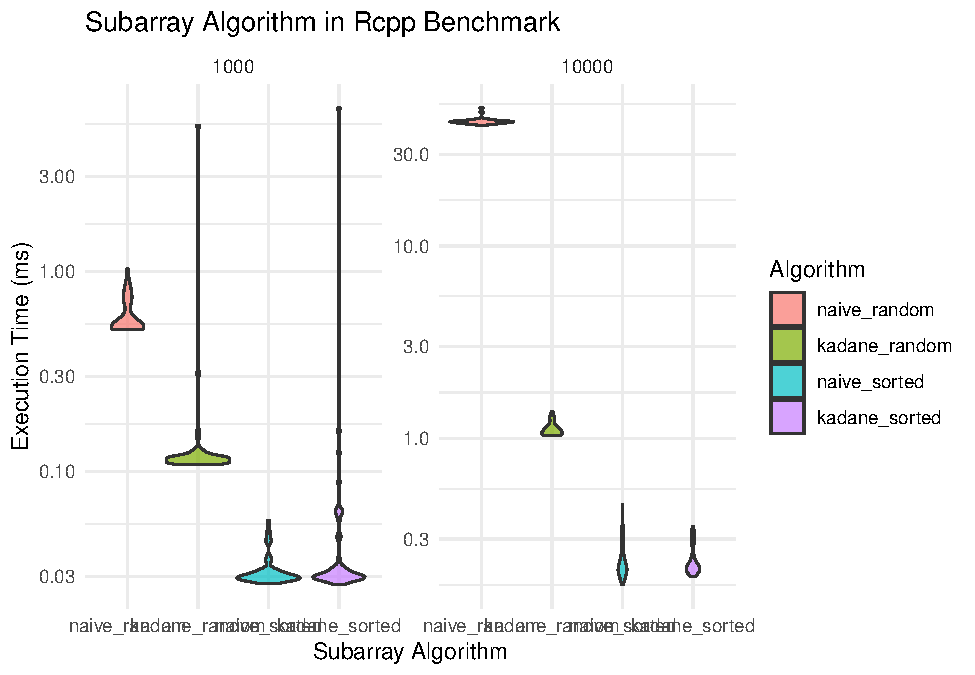
\includegraphics{MaxSubarray1D_files/figure-latex/benchmark2-1.pdf}

\begin{verbatim}
## # A tibble: 8 x 10
##       n expr       min_time q1_time median_time mean_time q3_time max_time type 
##   <dbl> <fct>         <dbl>   <dbl>       <dbl>     <dbl>   <dbl>    <dbl> <chr>
## 1  1000 naive_ran~   0.325   0.327       0.329     0.376   0.374    0.704  rand~
## 2  1000 kadane_ra~   0.0688  0.0698      0.0704    0.127   0.0713   2.88   rand~
## 3  1000 naive_sor~   0.0173  0.0185      0.0191    0.131   0.0200   5.43   sort~
## 4  1000 kadane_so~   0.0177  0.0185      0.0191    0.0206  0.0198   0.0658 sort~
## 5 10000 naive_ran~  26.4    27.3        27.8      27.9    28.6     31.2    rand~
## 6 10000 kadane_ra~   0.636   0.685       0.697     0.709   0.724    0.837  rand~
## 7 10000 naive_sor~   0.0951  0.146       0.155     0.165   0.173    0.276  sort~
## 8 10000 kadane_so~   0.0948  0.145       0.156     0.163   0.173    0.341  sort~
## # i 1 more variable: algo <chr>
\end{verbatim}

Pour n = 1000, le temps d'exécution est plus rapide que pour n = 10000.
Kadane est toujours plus rapide que Naïf, avec un écart plus important à
n = 10000. Lorsque les tableaux sont triés, Naïf et Kadane sont beaucoup
plus rapides, avec un écart réduit entre les deux.

\end{document}
